%% ============================================================
%%  Toggle solutions: set \showsolutionstrue to show, false to hide
%% ============================================================
\newif\ifshowsolutions
\showsolutionstrue   %% <-- change to \showsolutionsfalse to hide solutions

\documentclass[12pt]{article}

\usepackage{fancyhdr}
\usepackage{lastpage}
\usepackage{float}
\usepackage{tikz}
\usepackage{amsmath}
\usepackage{pgfplots}
\usepackage{multirow}
\usepackage{caption}
\usepackage{amssymb}
\usepackage{hyperref}
\usepackage{subcaption}
\usepackage{xcolor}
\usepackage{mdframed}
\usepackage{verbatim}
\usetikzlibrary{automata,positioning,arrows}
\usepackage[top=01in, left=0.75in,right=0.75in,headsep=1mm,footskip=.5in]{geometry}

\usepackage{algorithm}
\usepackage{algpseudocode}

\DeclareMathOperator*{\argmax}{arg\,max}
\DeclareMathOperator*{\argmin}{arg\,min}

%% Solution environment -- toggled by \ifshowsolutions
\newmdenv[
  backgroundcolor=blue!6,
  linecolor=blue!40,
  linewidth=1pt,
  topline=true, bottomline=true, leftline=true, rightline=true,
  innerleftmargin=8pt, innerrightmargin=8pt,
  innertopmargin=6pt, innerbottommargin=6pt,
  skipabove=6pt, skipbelow=6pt
]{solutionbox}

\newenvironment{solution}{%
  \ifshowsolutions\begin{solutionbox}\noindent\textbf{\color{blue!70!black}Solution.}\quad\fi
  \ifshowsolutions\else\expandafter\comment\fi
}{%
  \ifshowsolutions\end{solutionbox}\fi
  \ifshowsolutions\else\expandafter\endcomment\fi
}

\pagestyle{fancy}
\let\headrule\empty
\let\footrule\empty
\lfoot{ROB\,311\,H1, Winter 2026}
\cfoot{Page \thepage\space of \pageref{LastPage}}
\rfoot{Practice Problems - Part 1}

\begin{document}

\begin{center}\large
  UNIVERSITY OF TORONTO\\
  Faculty of Applied Science and Engineering\\[1.75ex]
  Institute of Aerospace Studies\\[1.75ex]
  \textbf{Practice Problems - Part 1} \\
  \textbf{{ROB\,311\,H1}} \\[4mm]
  Winter 2026

  \vspace{3cm}
  \textbf{Chandra Gummaluru} \\
\href{https://chandra-gummaluru.github.io}{\texttt{chandra-gummaluru.github.io}}
\end{center}

\clearpage

\subsection*{Search Problems}
\begin{enumerate}
\item Consider a search problem over the graph shown below. Assume the initial state is $s_0 = A$ and the goal set is $\mathcal{G} = \lbrace G \rbrace $. For each algorithm, provide the path $p$ (as a sequence of states), and its cost, $\textsf{cst}(p)$. Break ties alphabetically. Use $\texttt{N/A}$ if the algorithm will not terminate.
    \begin{figure}[H]
        \centering
         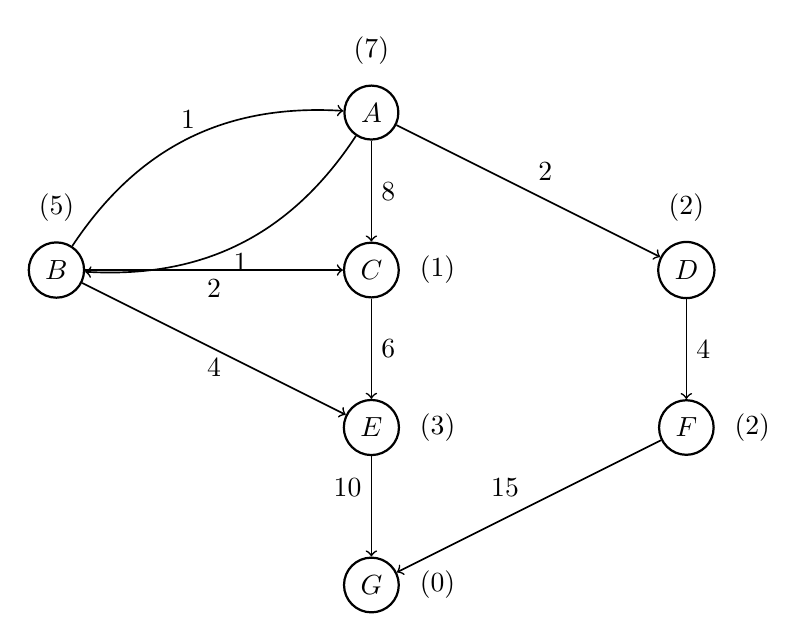
\begin{tikzpicture}[
            auto,
            node distance = 2cm,
            semithick
        ]

        \tikzstyle{every state}=[
            draw = black,
            thick,
            fill = white,
            minimum size = 4mm
        ]

        \node[state] (a) at (0, 0) {$A$};

        \node[state] (b) at (-4, -2) {$B$};
        \node[state] (c) at (0, -2) {$C$};
        \node[state] (d) at (4, -2) {$D$};

        \node[state] (e) at (0, -4) {$E$};
        \node[state] (f) at (4, -4) {$F$};

        \node[state] (g) at (0, -6) {$G$};

        \path[->] (a) edge[bend left] node [below] {$1$} (b);
        \path[->] (b) edge[bend left] node [above] {$1$} (a);
        \path[->] (a) edge node {$8$} (c);
        \path[->] (a) edge node {$2$} (d);

        \path[->] (b) edge node[below] {$4$} (e);
        \path[->] (b) edge node[below] {$2$} (c);
        \path[->] (c) edge node {$6$} (e);
        \path[->] (d) edge node {$4$} (f);

        \path[->] (e) edge node [above left] {$10$} (g);
        \path[->] (f) edge node [above left] {$15$} (g);

        \node [above=0.125cm of a] {$(7)$};
        \node [above=0.125cm of b] {$(5)$};
        \node [above=0.125cm of d] {$(2)$};
        \node [right=0.125cm of c] {$(1)$};
        \node [right=0.125cm of e] {$(3)$};
        \node [right=0.125cm of f] {$(2)$};
        \node [right=0.125cm of g] {$(0)$};

            \end{tikzpicture}
    \end{figure}

\begin{enumerate}
\item Breadth-First Search

\begin{solution}
  BFS expands nodes layer by layer (ignoring edge costs). Starting from $A$:
  \begin{itemize}
    \item Layer 0: expand $A$ $\to$ frontier $\{B, C, D\}$.
    \item Layer 1: expand $B$ $\to$ adds $A$ (already seen), $C$ (already seen), $E$; expand $C$ $\to$ adds $E$ (already queued); expand $D$ $\to$ adds $F$.
    \item Layer 2: expand $E$ $\to$ adds $G$; $G$ is the goal.
  \end{itemize}
  The first path to reach $G$ via BFS is $A \to B \to E \to G$ with cost $1+4+10 = \mathbf{15}$.
\end{solution}

\item Depth-First Search

\begin{solution}
  DFS without any cycle checking will follow $A \to B \to A \to B \to \cdots$ indefinitely along the mutual edge. The algorithm \textbf{does not terminate}: $\texttt{N/A}$.
\end{solution}

\item Depth-First Search w/ Inter-Path Cycle Checking

\begin{solution}
  Inter-path (closed-set) cycle checking prevents re-expanding any previously visited node. DFS explores alphabetically:
  \[
    A \;\to\; B \;\to\; E \;\to\; G.
  \]
  ($A$ is marked visited before expanding $B$, so the $B\to A$ back-edge is pruned.) Path: $A \to B \to E \to G$, cost $= 1+4+10 = \mathbf{15}$.
\end{solution}

\item Cheapest-First Search

\begin{solution}
  CFS (uniform-cost search) expands the node with the lowest accumulated cost $g$. Expansion order (ties broken alphabetically):
  \begin{center}
  \begin{tabular}{cll}
    Step & Expanded & Frontier (selected cost) \\\hline
    1 & $A$ $(g=0)$ & $B(1),\;D(2),\;C(8)$ \\
    2 & $B$ $(g=1)$ & $D(2),\;C(3),\;E(5),\;C(8)$ \\
    3 & $D$ $(g=2)$ & $C(3),\;E(5),\;F(6),\;C(8)$ \\
    4 & $C$ $(g=3)$ & $E(5),\;F(6),\;E(9),\;C(8)$ \\
    5 & $E$ $(g=5)$ & $F(6),\;G(15),\;E(9),\;C(8)$ \\
    6 & $F$ $(g=6)$ & $G(15),\;E(9),\;C(8),\;G(21)$ \\
    7 & $C$ $(g=8)$ & skip (already expanded) \\
    8 & $E$ $(g=9)$ & skip \\
    9 & $G$ $(g=15)$ & \textbf{goal}
  \end{tabular}
  \end{center}
  Path: $A \to B \to E \to G$, cost $= \mathbf{15}$.
\end{solution}

\item A* Search

\begin{solution}
  $f(n) = g(n) + h(n)$. Expansion order:
  \begin{center}
  \begin{tabular}{cll}
    Step & Expanded & Notable frontier entries (f-values) \\\hline
    1 & $A$ $(f=7)$ & $B(f=6),\;D(f=4),\;C(f=9)$ \\
    2 & $D$ $(f=4)$ & $B(f=6),\;F(f=8),\;C(f=9)$ \\
    3 & $B$ $(f=6)$ & $C(f=4),\;E(f=8),\;F(f=8),\;C(f=9)$ \\
    4 & $C$ $(g=3,f=4)$ & $E(f=8),\;F(f=8),\;E(f=12),\;C(f=9)$ \\
    5 & $E$ $(g=5,f=8)$ & $F(f=8),\;G(f=15),\;E(f=12)$ \\
    6 & $F$ $(g=6,f=8)$ & $G(f=15),\;G(f=21),\;\ldots$ \\
    7 & $G$ $(g=15,f=15)$ & \textbf{goal}
  \end{tabular}
  \end{center}
  At step 5, $E$ (via $A\!\to\!B\!\to\!E$) and $F$ tie at $f=8$; $E$ is chosen alphabetically. Path: $A \to B \to E \to G$, cost $= \mathbf{15}$.
\end{solution}

\item A* Search w/ Intra-Path Cycle Checking

\begin{solution}
  Intra-path cycle checking (no closed set) only prevents revisiting a node on the \emph{current path}. Because the optimal path $A\!\to\!B\!\to\!E\!\to\!G$ contains no cycles, the result is identical to standard A*. Path: $A \to B \to E \to G$, cost $= \mathbf{15}$.
\end{solution}

\item Nearest-First Search

\begin{solution}
  Greedy best-first expands the node with the smallest heuristic $h$. Expansion order:
  \begin{center}
  \begin{tabular}{cll}
    Step & Expanded $(h)$ & Frontier \\\hline
    1 & $A\;(h=7)$ & $B(5),\;C(1),\;D(2)$ \\
    2 & $C\;(h=1)$ & $B(5),\;D(2),\;E(3)$ \\
    3 & $E\;(h=3)$ & $B(5),\;D(2),\;G(0)$ \\
    4 & $G\;(h=0)$ & \textbf{goal}
  \end{tabular}
  \end{center}
  Path: $A \to C \to E \to G$, cost $= 8+6+10 = \mathbf{24}$.
\end{solution}

\item Nearest-First Search w/ Intra-Path Cycle Checking

\begin{solution}
  The path $A\!\to\!C\!\to\!E\!\to\!G$ contains no repeated nodes, so intra-path cycle checking does not change the result. Path: $A \to C \to E \to G$, cost $= \mathbf{24}$.
\end{solution}

\end{enumerate}
\end{enumerate}

\clearpage

\subsection*{Probabilistic Inference}
\begin{enumerate}
  \item \textit{Dependence Separation}. Consider the Bayesian network shown below:
        \begin{figure}[H]
          \centering
          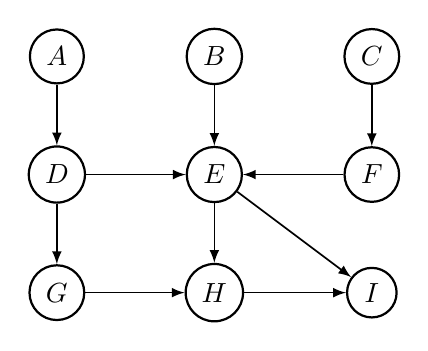
\begin{tikzpicture}[
              auto,
              node distance = 2cm,
              semithick
            ]

            \tikzstyle{every state}=[
            draw = black,
            thick,
            fill = white,
            minimum size = 4mm
            ]


            \node[state] (a) at (-2, 0) {$A$};
            \node[state] (b) at (0, 0) {$B$};
            \node[state] (c) at (2, 0) {$C$};
            \node[state] (d) at (-2, -1.5) {$D$};
            \node[state] (e) at (0, -1.5) {$E$};
            \node[state] (f) at (2, -1.5) {$F$};
            \node[state] (g) at (-2, -3) {$G$};
            \node[state] (h) at (0, -3) {$H$};
            \node[state] (i) at (2, -3) {$I$};

            \path[-latex] (b) edge node {} (e);
            \path[-latex] (c) edge node {} (f);
            \path[-latex] (d) edge node {} (e);
            \path[-latex] (d) edge node {} (g);
            \path[-latex] (e) edge node {} (h);
            \path[-latex] (e) edge node {} (i);
            \path[-latex] (f) edge node {} (e);
            \path[-latex] (g) edge node {} (h);
            \path[-latex] (h) edge node {} (i);
            \path[-latex] (a) edge node {} (d);
          \end{tikzpicture}
        \end{figure}
        \begin{enumerate}
            \item Determine whether each of the following statements are \textbf{True} or \textbf{False}.
        \begin{enumerate}
          \item It is guaranteed that $A \perp C$

          \begin{solution}
            \textbf{True.} Every undirected path from $A$ to $C$ passes through $E$, which is a collider ($D\!\to\!E\!\leftarrow\!F\!\leftarrow\!C$). Since $E$ is not observed and no descendant of $E$ is observed, the collider blocks this path. No other path connects $A$ to $C$, so $A$ and $C$ are d-separated and therefore marginally independent.
          \end{solution}

          \item It is guaranteed that $B \perp C | I$

          \begin{solution}
            \textbf{False.} Consider the path $B\!\to\!E\!\leftarrow\!F\!\leftarrow\!C$. The node $E$ is a collider on this path. Conditioning on $I$, a descendant of $E$ (via $E\!\to\!I$), opens the collider and activates this path. Hence $B$ and $C$ are not d-separated given $I$.
          \end{solution}

          \item It is guaranteed that $D \perp I | \lbrace E, G \rbrace$

          \begin{solution}
            \textbf{True.} Every path from $D$ to $I$ must pass through either $E$ or $G$:
            \begin{itemize}
              \item $D\!\to\!E\!\to\!I$: blocked by observing $E$ (chain).
              \item $D\!\to\!E\!\to\!H\!\to\!I$: blocked by observing $E$ (chain).
              \item $D\!\to\!G\!\to\!H\!\to\!I$: blocked by observing $G$ (chain).
            \end{itemize}
            All paths are blocked, so $D \perp I \mid \{E, G\}$.
          \end{solution}

          \item It is guaranteed that $C \perp H | G$

          \begin{solution}
            \textbf{False.} The path $C\!\to\!F\!\to\!E\!\to\!H$ is a chain; $G$ does not lie on this path, so conditioning on $G$ does not block it. Hence $C$ and $H$ are not d-separated given $G$.
          \end{solution}
        \end{enumerate}
    \clearpage
  \item \textit{Exact Inference on a Bayesian Network via Variable Elimination}. Consider the following Bayesian network, where $A, B, C, D$ are binary random variables over $\lbrace 0, 1 \rbrace$.
        \begin{figure}[H]
          \centering
          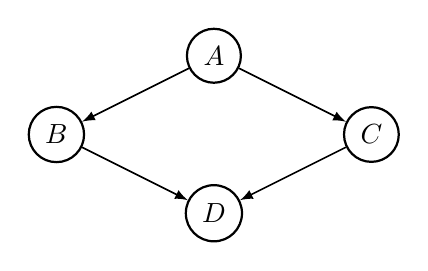
\begin{tikzpicture}[
              auto,
              node distance = 2cm,
              semithick
            ]

            \tikzstyle{every state}=[
            draw = black,
            thick,
            fill = white,
            minimum size = 4mm
            ]


            \node[state] (A) at (0, 0) {$A$};
            \node[state] (B) at (-2, -1) {$B$};
            \node[state] (C) at (2, -1) {$C$};
            \node[state] (D) at (0, -2) {$D$};

            \path[-latex] (A) edge node {} (B);
            \path[-latex] (A) edge node {} (C);
            \path[-latex] (B) edge node {} (D);
            \path[-latex] (C) edge node {} (D);
          \end{tikzpicture}
        \end{figure}
        The conditional probability tables for the network are:
        \begin{table}[H]
          \centering
          \begin{tabular}{|c|}
            \hline
            $P(A=1)$ \\\hline
            0.1      \\\hline
          \end{tabular}
        \end{table}
        \vspace{-1em}
        \begin{table}[H]
          \centering
          \begin{tabular}{|r|c|}
            \hline
            $A$ & $P(B=1|A)$ \\\hline
            $0$ & 0.4        \\\hline
            $1$ & 0.5        \\\hline
          \end{tabular}
          \hspace{1cm}
          \begin{tabular}{|r|c|}

            \hline
            $A$ & $P(C=1|A)$ \\\hline
            $0$ & 0.2        \\\hline
            $1$ & 0.4        \\\hline
          \end{tabular}
        \end{table}
        \vspace{-1em}
        \begin{table}[H]
          \centering
          \begin{tabular}{|r|r|c|}

            \hline
            $B$ & $C$ & $P(D=1|B,C)$ \\\hline
            $0$ & $0$ & 0.5          \\\hline
            $0$ & $1$ & 0.2          \\\hline
            $1$ & $0$ & 0.5          \\\hline
            $1$ & $1$ & 0.4          \\\hline
          \end{tabular}
        \end{table}
        \begin{enumerate}
          \item Find the exact value of $P(A=0|C=0)$.

          \begin{solution}
            By Bayes' rule:
            \[
              P(A=0\mid C=0) = \frac{P(C=0\mid A=0)\,P(A=0)}{P(C=0)}.
            \]
            \begin{align*}
              P(C=0) &= P(C=0\mid A=0)P(A=0) + P(C=0\mid A=1)P(A=1)\\
                     &= 0.8\times 0.9 + 0.6\times 0.1 = 0.72 + 0.06 = 0.78.\\[4pt]
              P(A=0\mid C=0) &= \frac{0.8\times 0.9}{0.78} = \frac{0.72}{0.78} = \frac{12}{13} \approx 0.923.
            \end{align*}
          \end{solution}

          \item Find the exact value of $P(D=1|C=0)$.

          \begin{solution}
            Marginalise over $A$ and $B$:
            \[
              P(D=1\mid C=0) = \frac{\displaystyle\sum_{a}\sum_{b} P(D=1\mid B=b, C=0)\,P(B=b\mid A=a)\,P(A=a)}{P(C=0)}.
            \]
            For $A=0$ ($P=0.9$):
            \[
              \sum_{b} P(D=1\mid b,0)\,P(b\mid 0)
              = 0.5\times 0.6 + 0.5\times 0.4 = 0.30 + 0.20 = 0.50.
            \]
            For $A=1$ ($P=0.1$):
            \[
              \sum_{b} P(D=1\mid b,0)\,P(b\mid 1)
              = 0.5\times 0.5 + 0.5\times 0.5 = 0.25 + 0.25 = 0.50.
            \]
            Numerator $= 0.9\times 0.50 + 0.1\times 0.50 = 0.45 + 0.05 = 0.50$.
            \[
              P(D=1\mid C=0) = \frac{0.50}{0.78} = \frac{25}{39} \approx 0.641.
            \]
          \end{solution}
        \end{enumerate}
        \clearpage
  \item \textit{Approximate Inference on Bayesian Networks via Sampling}. Consider the following Bayesian network, where $A, B, C, D$ are binary random variables over $\lbrace 0, 1 \rbrace$.
        \begin{figure}[H]
          \centering
          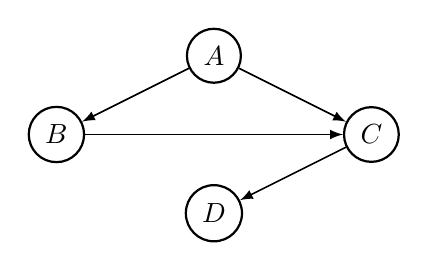
\begin{tikzpicture}[
              auto,
              node distance = 2cm,
              semithick
            ]

            \tikzstyle{every state}=[
            draw = black,
            thick,
            fill = white,
            minimum size = 4mm
            ]


            \node[state] (A) at (0, 0) {$A$};
            \node[state] (B) at (-2, -1) {$B$};
            \node[state] (C) at (2, -1) {$C$};
            \node[state] (D) at (0, -2) {$D$};

            \path[-latex] (A) edge node {} (B);
            \path[-latex] (A) edge node {} (C);
            \path[-latex] (C) edge node {} (D);
            \path[-latex] (B) edge node {} (C);
          \end{tikzpicture}
        \end{figure}
        The conditional probability tables for the network are:
        \begin{table}[H]
          \centering
          \begin{tabular}{|c|}
            \hline
            $P(A=1)$ \\\hline
            0.1      \\\hline
          \end{tabular}
        \end{table}
        \vspace{-1em}
        \begin{table}[H]
          \centering
          \begin{tabular}{|r|c|}
            \hline
            $A$ & $P(B=1|A)$ \\\hline
            $0$ & 0.4        \\\hline
            $1$ & 0.5        \\\hline
          \end{tabular}
          \hspace{1cm}
          \begin{tabular}{|r|r|c|}

            \hline
            $A$ & $B$ & $P(C=1|A,B)$ \\\hline
            $0$ & $0$ & 0.5          \\\hline
            $0$ & $1$ & 0.2          \\\hline
            $1$ & $0$ & 0.5          \\\hline
            $1$ & $1$ & 0.4          \\\hline
          \end{tabular}
        \end{table}
        \vspace{-1em}
        \begin{table}[H]
          \centering
          \begin{tabular}{|r|c|}

            \hline
            $C$ & $P(D=1|C)$ \\\hline
            $0$ & 0.2        \\\hline
            $1$ & 0.4        \\\hline
          \end{tabular}
        \end{table}
        The goal is to approximate the value of $P(D=1|C=0)$ by sampling the network.
        \begin{enumerate}
          \item Recall that to sample a random variable, $X$, its parents, $\text{pts}(X)$ should have already been sampled. If $X$ is binary, and its parents have already been sampled, we can sample $X$ by first sampling a uniform random variable over $[0, 1]$, say $V$, and defining the sampled value of $X$ to be $\mathbb{I}[V \leq \mathbb{P}[X = 1 | \text{pts}(X)]]$. Suppose a random number generator produces the following output for the first 10 IID samples of $V$:
                \[0.2, 0.3, 0.3, 0.3, 0.4, 0.6, 0.4, 0.4, 0.9, 1.0\]
                Provide the first sample of the network using a depth-first search ordering starting with $A$ (breaking ties alphabetically).

          \begin{solution}
            A DFS ordering starting from $A$ (ties alphabetical) visits the variables in the order $A, B, C, D$.

            \begin{center}
            \begin{tabular}{cccc}
              Variable & Condition & Threshold $P(X=1\mid\cdot)$ & $V$ used \\\hline
              $A$ & --- & $0.1$ & $0.2 > 0.1 \Rightarrow A=0$ \\
              $B$ & $A=0$ & $0.4$ & $0.3 \leq 0.4 \Rightarrow B=1$ \\
              $C$ & $A=0,B=1$ & $0.2$ & $0.3 > 0.2 \Rightarrow C=0$ \\
              $D$ & $C=0$ & $0.2$ & $0.3 > 0.2 \Rightarrow D=0$ \\
            \end{tabular}
            \end{center}

            First sample: $(A, B, C, D) = (0, 1, 0, 0)$.
          \end{solution}

        \clearpage
          \item Suppose the network is sampled several times, and the results are as those shown in the table below:
                \begin{table}[H]
                  \centering
                  \begin{tabular}{|c|c|c|c|c|}
                    \hline
                    $A$ & $B$ & $C$ & $D$ \\
                    \hline
                    1   & 0   & 1   & 1   \\\hline
                    1   & 0   & 1   & 1   \\\hline
                    0   & 1   & 0   & 1  \\\hline
                    1   & 1   & 0   & 1    \\\hline
                    1   & 0   & 1   & 1  \\\hline
                    0   & 1   & 0   & 1   \\\hline
                    0   & 0   & 0   & 1   \\\hline
                    0   & 1   & 0   & 1    \\\hline
                    1   & 1   & 1   & 0    \\\hline
                    0   & 0   & 0   & 0    \\\hline
                    1   & 0   & 0   & 1   \\\hline
                    1   & 1   & 0   & 1   \\\hline
                    0   & 1   & 0   & 1    \\\hline
                    0   & 0   & 0   & 1   \\\hline
                    1   & 0   & 0   & 1    \\\hline
                    0   & 1   & 0   & 0     \\\hline
                    0   & 0   & 1   & 1    \\\hline
                    1   & 0   & 0   & 0   \\\hline
                    0   & 0   & 0   & 1    \\\hline
                    1   & 0   & 0   & 1    \\\hline
                  \end{tabular}
                \end{table}
                Approximate the value of $P(D=1|C=0)$ using these samples. Do NOT include the samples from (i).

          \begin{solution}
            Filter to rows where $C=0$: rows 3, 4, 6, 7, 8, 10, 11, 12, 13, 14, 15, 16, 18, 19, 20.
            That gives 15 samples with $C=0$. Of these, $D=1$ in rows 3, 4, 6, 7, 8, 11, 12, 13, 14, 15, 19, 20 -- a total of 12 samples.
            \[
              P(D=1\mid C=0) \approx \frac{12}{15} = \frac{4}{5} = 0.8.
            \]
          \end{solution}
        \end{enumerate}
\end{enumerate}
\end{enumerate}
\clearpage
\subsection*{Markov Decision Processes}
\begin{enumerate}
  \item \textit{Finding the Optimal Policy of an MDP}. Consider an MDP with $\mathcal{S} = \lbrace 1, 2, 3 \rbrace$ and $\mathcal{A} = \lbrace \text{A}, \text{B} \rbrace$ as shown below:
   \begin{figure}[H]
          \centering
          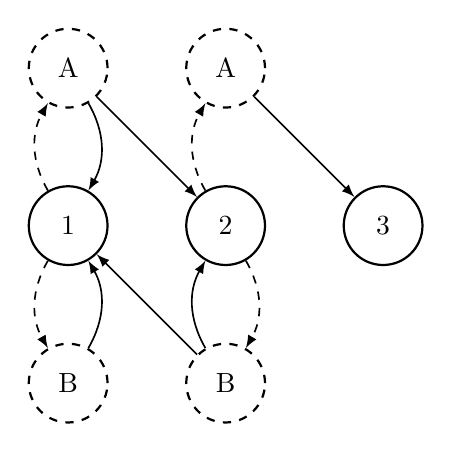
\begin{tikzpicture}[
              auto,
              node distance = 2cm,
              semithick
            ]

            \tikzstyle{every state}=[
            draw = black,
            thick,
            fill = white,
            minimum size = 10mm,
            ]

            \node[state] at (4,0) (s3) {$3$};
            \node[state] at (0,0) (s1) {$1$};
            \node[state] at (2,0) (s2) {$2$};

            \node[state, dashed] at (0,2) (a11) {A};
            \node[state, dashed] at (0,-2) (a12) {B};

            \node[state, dashed] at (2,2) (a21) {A};
            \node[state, dashed] at (2,-2) (a22) {B};

            \path[-latex, dashed, bend left] (s1) edge (a11);
            \path[-latex, dashed, bend right] (s1) edge (a12);

            \path[-latex, bend left] (a11) edge (s1);
            \path[-latex] (a11) edge (s2);
            \path[-latex, bend right] (a12) edge (s1);


            \path[-latex, dashed, bend left] (s2) edge (a21);
            \path[-latex, dashed, bend left] (s2) edge (a22);

            \path[-latex] (a21) edge (s3);

            \path[-latex, bend left] (a22) edge (s2);
            \path[-latex] (a22) edge (s1);

          \end{tikzpicture}
        \end{figure}
    Assume the following:
    \begin{itemize}
        \item $p(\cdot|s,a)$ is uniform for any fixed $s$ and $a$
        \item $r(s,\text{A},s') = +2$ if $s' \neq 3$ and $r(s,\text{A},3) = -10$
        \item $r(s,\text{B},s') = +1$
    \end{itemize}
    \begin{enumerate}
        \item Let $q(\cdot,\cdot) \equiv 0$ initially. Use the recurrence describing the optimal Q-values (under $\gamma = 0.5$) to update $q$. Then, update $q$ again. List the resulting Q-values.

        \begin{solution}
          From the diagram, the transitions are:
          \begin{itemize}
            \item $(1,\mathrm{A})$: goes to $\{1, 2\}$ with probability $\tfrac{1}{2}$ each.
            \item $(1,\mathrm{B})$: goes to $\{1\}$ with probability $1$.
            \item $(2,\mathrm{A})$: goes to $\{3\}$ with probability $1$.
            \item $(2,\mathrm{B})$: goes to $\{1, 2\}$ with probability $\tfrac{1}{2}$ each.
          \end{itemize}
          State 3 has no outgoing actions; $\max_{a'}q(3,a') = 0$ throughout.

          The optimal Q-value recurrence is:
          \[
            q(s,a) = \sum_{s'} p(s'\mid s,a)\bigl[r(s,a,s') + \gamma\max_{a'}q(s',a')\bigr].
          \]

          \textbf{Iteration 1} (from $q \equiv 0$):
          \begin{align*}
            q(1,\mathrm{A}) &= \tfrac{1}{2}[+2 + 0] + \tfrac{1}{2}[+2 + 0] = 2.00\\
            q(1,\mathrm{B}) &= 1\cdot[+1 + 0] = 1.00\\
            q(2,\mathrm{A}) &= 1\cdot[-10 + 0] = -10.00\\
            q(2,\mathrm{B}) &= \tfrac{1}{2}[+1 + 0] + \tfrac{1}{2}[+1 + 0] = 1.00
          \end{align*}

          \textbf{Iteration 2} (from values above):
          \begin{align*}
            q(1,\mathrm{A}) &= \tfrac{1}{2}\bigl[2 + 0.5\cdot\max(2,1)\bigr] + \tfrac{1}{2}\bigl[2 + 0.5\cdot\max(-10,1)\bigr]\\
                            &= \tfrac{1}{2}(2+1) + \tfrac{1}{2}(2+0.5) = 1.5 + 1.25 = 2.75\\[4pt]
            q(1,\mathrm{B}) &= 1\cdot\bigl[1 + 0.5\cdot\max(2,1)\bigr] = 1 + 1 = 2.00\\[4pt]
            q(2,\mathrm{A}) &= 1\cdot[-10 + 0.5\cdot 0] = -10.00\\[4pt]
            q(2,\mathrm{B}) &= \tfrac{1}{2}\bigl[1 + 0.5\cdot\max(-10,1)\bigr] + \tfrac{1}{2}\bigl[1 + 0.5\cdot\max(2,1)\bigr]\\
                            &= \tfrac{1}{2}(1+0.5) + \tfrac{1}{2}(1+1) = 0.75 + 1 = 1.75
          \end{align*}

          \begin{center}
          \begin{tabular}{|c|c|c|}
            \hline
            $s$ & $a$ & $q(s,a)$ after 2 iterations \\\hline
            1 & A & 2.75 \\\hline
            1 & B & 2.00 \\\hline
            2 & A & $-10.00$ \\\hline
            2 & B & 1.75 \\\hline
          \end{tabular}
          \end{center}
        \end{solution}

            \item Suppose that the Q-values (under $\gamma = 0.5$) were estimated to be those shown in the table below:
                \begin{table}[H]
                  \centering
                  \begin{tabular}{|c|c|c|}
                    \hline
                    $s$   & $a$   & $q(s,a)$ \\\hline
                    $1$ & A & 2.14         \\\hline
                    $1$ & B & 2.21         \\\hline
                    $2$ & A & 3.42         \\\hline
                    $2$ & B & 3.12         \\\hline
                  \end{tabular}
                \end{table}
    List the values of the optimal policy $\pi(\cdot|\cdot)$.

    \begin{solution}
      The greedy (optimal) policy selects the action with the highest Q-value in each state:
      \begin{align*}
        \pi(1) &= \argmax_{a}\, q(1,a) = \mathrm{B} \quad (2.21 > 2.14),\\
        \pi(2) &= \argmax_{a}\, q(2,a) = \mathrm{A} \quad (3.42 > 3.12).
      \end{align*}
      State 3 is absorbing with no outgoing actions, so no policy is defined there.
    \end{solution}
    \end{enumerate}
    \clearpage
        \item \textit{Updating Beliefs in a POMDP}: Consider the following 3-state Markov decision process:
        \begin{figure}[H]
          \centering
          \begin{tikzpicture}[
              auto,
              node distance = 2cm,
              semithick
            ]

            \tikzstyle{every state}=[
            draw = black,
            thick,
            fill = white,
            minimum size = 10mm,
            ]

            \node[state] at (0,-1) (s2) {$3$};
            \node[state] at (-3,4) (s0) {$1$};
            \node[state] at (3,4) (s1) {$2$};

            \node[state, dashed] at (-5,2) (a10) {A};
            \node[state, dashed] at (-1.5,2) (a20) {B};

            \node[state, dashed] at (1.5,2) (a11) {A};
            \node[state, dashed] at (5,2) (a21) {B};

            \node[state, dashed] at (-3,0.5) (a12) {A};
            \node[state, dashed] at (0, -2.5) (a22) {B};


            \path[-latex, dashed, bend left] (s0) edge(a10);
            \path[-latex, dashed] (s0) edge (a20);

            \path[-latex, dashed, bend left] (s1) edge (a11);
            \path[-latex, dashed, bend left] (s1) edge (a21);

            \path[-latex, dashed, bend right] (s2) edge (a12);
            \path[-latex, dashed, bend right] (s2) edge (a22);

            \path[-latex, bend left] (a10) edge node[above left] {$0.5$}  (s0);
            \path[-latex, bend right=50] (a10) edge node[below left] {$0.5$}  (s2);

            \path[-latex] (a20) edge node[above right] {$1.0$} (s2);

            \path[-latex, bend right] (a11) edge node[above right] {$0.7$}  (s0);
            \path[-latex, bend left] (a11) edge node[left] {$0.1$}  (s1);
            \path[-latex] (a11) edge node[below right] {$0.2$}  (s2);

            \path[-latex, bend left=50] (a21) edge node[right below] {$0.05$} (s2);
            \path[-latex, bend left] (a21) edge node[left below] {$0.95$} (s1);

            \path[-latex] (a12) edge node[left] {$0.4$}  (s0);
            \path[-latex, bend right] (a22) edge node[right] {$0.4$} (s2) ;
            \path[-latex] (a12) edge node[below left] {$0.6$}  (s2);

            \draw[-latex, rounded corners=1cm] (a22) -- (-5.75,-2.5) node[below, midway] {$0.3$} -- (-5.75,4) -- (s0);
            \draw[-latex, rounded corners=1cm] (a22) -- (5.75,-2.5) node[below, midway] {$0.3$} -- (5.75,4) -- (s1);

          \end{tikzpicture}
        \end{figure}
        Suppose the state cannot be measured directly. Instead, a measurement (correspond to the state) is taken. Given the state $s \in \lbrace 1, 2, 3 \rbrace$, the measurement, $O$, is a random variable over $\lbrace 1, 2, 3 \rbrace$, distributed according to $m(o|s)$. If the process is in state $x \in \lbrace 1, 2, 3 \rbrace$, the measurement will correspond to the $x$ with a probability of $1 - 0.2x$, and one of the other two states with equal probability.
\begin{enumerate}
  \item Suppose the prior belief in the initial state is uniform across the states. If the measurement of the initial state corresponds to State 1, what is the posterior probability that the process is actually in State 1?

  \begin{solution}
    The observation model gives:
    \[
      m(o=s \mid s) = 1 - 0.2s, \qquad
      m(o \neq s \mid s) = \frac{0.2s}{2} = 0.1s \text{ (for each of the other two values)}.
    \]
    Explicitly for observation $O=1$:
    \begin{align*}
      m(O=1 \mid s=1) &= 1 - 0.2 = 0.8,\\
      m(O=1 \mid s=2) &= 0.1\times 2 = 0.2,\\
      m(O=1 \mid s=3) &= 0.1\times 3 = 0.3.
    \end{align*}
    With uniform prior $P(s) = \tfrac{1}{3}$:
    \[
      P(O=1) = \frac{0.8 + 0.2 + 0.3}{3} = \frac{1.3}{3}.
    \]
    \[
      P(s=1 \mid O=1) = \frac{m(O=1\mid s=1)\,P(s=1)}{P(O=1)}
                      = \frac{0.8/3}{1.3/3} = \frac{0.8}{1.3} = \frac{8}{13} \approx 0.615.
    \]
  \end{solution}

  \item Ignoring the answer to (a), suppose the belief in the state distribution after the initial observation is $60\%$ for State 1, and evenly split between the other two states. If the agent takes action $\text{A}$, and measures the resulting state to be State 2, what is the probability that the agent is actually in State 2?

  \begin{solution}
    Prior belief: $b(1)=0.6,\;b(2)=0.2,\;b(3)=0.2$.

    \textbf{Step 1: Predict.} Propagate through the transition model under action $\mathrm{A}$:
    \begin{align*}
      P(s'=1) &= b(1)\,p(1\mid 1,\mathrm{A}) + b(2)\,p(1\mid 2,\mathrm{A}) + b(3)\,p(1\mid 3,\mathrm{A})\\
              &= 0.6\times 0.5 + 0.2\times 0.7 + 0.2\times 0.4 = 0.30+0.14+0.08 = 0.52,\\
      P(s'=2) &= 0.6\times 0 + 0.2\times 0.1 + 0.2\times 0 = 0.02,\\
      P(s'=3) &= 0.6\times 0.5 + 0.2\times 0.2 + 0.2\times 0.6 = 0.30+0.04+0.12 = 0.46.
    \end{align*}

    \textbf{Step 2: Update.} Apply observation $O=2$ using the observation model:
    \begin{align*}
      P(s'=1,O=2) &= 0.52\times m(O=2\mid 1) = 0.52\times 0.1 = 0.052,\\
      P(s'=2,O=2) &= 0.02\times m(O=2\mid 2) = 0.02\times 0.6 = 0.012,\\
      P(s'=3,O=2) &= 0.46\times m(O=2\mid 3) = 0.46\times 0.3 = 0.138.
    \end{align*}
    Normalising constant: $0.052 + 0.012 + 0.138 = 0.202$.
    \[
      P(s'=2 \mid O=2) = \frac{0.012}{0.202} = \frac{6}{101} \approx 0.059.
    \]
  \end{solution}
  \end{enumerate}
    \item \textit{Tracing Q-Learning}. Consider an MDP with $\mathcal{S} = \lbrace 1, 2, 3 \rbrace$ and $\mathcal{A} = \lbrace \text{A}, \text{B} \rbrace$. The transition probabilities and rewards are unknown, but can be accurately simulated. Suppose $K = 2$ simulation episodes are performed with $l_{\text{max}} = 5$. The resulting paths are shown:
        \begin{table}[H]
            \centering
            \begin{tabular}{|c|l|}
                \hline
                 Ep. \# & Path  \\\hline
                 1 & $\langle (1,\text{A},3, +4),  (3,\text{A},3, +2),  (3,\text{B},2, -2), (2, \text{A}, 2, +2), (2,\text{A},2,+2)\rangle$ \\\hline
                 2 & $\langle (1,\text{B},3,+5),  (3,\text{A},2,-1),  (2,\text{B},3,-3), (3,\text{A},3,+2),(3,\text{A},3,+3)\rangle$ \\\hline
            \end{tabular}
        \end{table}
        If $\gamma = 0.5$, provide the estimated $q$-values using Q-learning.

        \begin{solution}
          Q-learning uses the update rule $q(s,a) \leftarrow r + \gamma \max_{a'} q(s',a')$ (learning rate $\alpha=1$, applied in the order transitions are observed). Initialise $q\equiv 0$.

          \textbf{Episode 1:}
          \begin{align*}
            (1,A,3,+4):\quad & q(1,A) \leftarrow 4 + 0.5\cdot\max_{a'}q(3,a') = 4 + 0 = 4.\\
            (3,A,3,+2):\quad & q(3,A) \leftarrow 2 + 0.5\cdot\max(0,0) = 2.\\
            (3,B,2,-2):\quad & q(3,B) \leftarrow -2 + 0.5\cdot\max_{a'}q(2,a') = -2 + 0 = -2.\\
            (2,A,2,+2):\quad & q(2,A) \leftarrow 2 + 0.5\cdot\max(0,0) = 2.\\
            (2,A,2,+2):\quad & q(2,A) \leftarrow 2 + 0.5\cdot\max(2,0) = 2 + 1 = 3.
          \end{align*}
          After Episode 1: $q(1,A)=4,\;q(2,A)=3,\;q(3,A)=2,\;q(3,B)=-2$; all others $= 0$.

          \textbf{Episode 2:}
          \begin{align*}
            (1,B,3,+5):\quad & q(1,B) \leftarrow 5 + 0.5\cdot\max(2,-2) = 5 + 1 = 6.\\
            (3,A,2,-1):\quad & q(3,A) \leftarrow -1 + 0.5\cdot\max(3,0) = -1 + 1.5 = 0.5.\\
            (2,B,3,-3):\quad & q(2,B) \leftarrow -3 + 0.5\cdot\max(0.5,-2) = -3 + 0.25 = -2.75.\\
            (3,A,3,+2):\quad & q(3,A) \leftarrow 2 + 0.5\cdot\max(0.5,-2) = 2 + 0.25 = 2.25.\\
            (3,A,3,+3):\quad & q(3,A) \leftarrow 3 + 0.5\cdot\max(2.25,-2) = 3 + 1.125 = 4.125.
          \end{align*}

          \textbf{Final Q-values:}
          \begin{center}
          \begin{tabular}{|c|c|c|}
            \hline
            $s$ & $a$ & $q(s,a)$ \\\hline
            1 & A & 4.000 \\\hline
            1 & B & 6.000 \\\hline
            2 & A & 3.000 \\\hline
            2 & B & $-2.750$ \\\hline
            3 & A & 4.125 \\\hline
            3 & B & $-2.000$ \\\hline
          \end{tabular}
          \end{center}
        \end{solution}
        \end{enumerate}
\end{document}